\subsection{Devops}
De nos jours, dans le domaine du numérique, nous livrons une large gamme de services grâce à des expériences numériques, et pour les améliorer, nous devons avoir le retour du client pour pouvoir proposer de nouveaux types d’expériences et de valeurs. Ce faisant, nous allons être plus compétitifs et nous aurons des nouveaux moyen d'interagir avec les clients.
Tout cela, nous pouvons le faire grâce à des bonnes pratiques pour rendre le travail beaucoup plus efficace, pour cela nous allons entrer dans le monde DevOps.

DevOps est avant tout une culture, des pratiques collaboratives et de l'automatisation qui alignent les équipes de développement et d'opération afin qu'elles puissent améliorer leur expérience client, répondre plus rapidement aux besoins et assurer l'innovation \cite{IsaacSacolick2016DrivingCulture}.

Cependant, cela n'est pas seulement une culture, DevOps involucre principalement un changement de base de comment nous gérons nos applications et comment nous les déployions, en investissant dans l'automation et en changeant les application héritées \cite{benjamin_wootton}.

Pour cette raison, quand nous parlons de DevOps, nous avons:

\begin{itemize}
\item L'automatisation de test.
\item Assurer des déploiements plus fréquents et plus fiables..
\item Avoir la clarté de rôles et des responsabilités.
\item Définir l'indicateur de performance \(KPI\) et sa portée.
\item Automatisation et surveillance.
\end{itemize}

Pour commencer, nous devons nous assurer que tous sont alignés sur ce que DevOps signifie et avec un défi et non à l’ensemble des pratiques DevOps.

Nous devons également rester concentrés sur l’assurance qualité (QA) en sachant qu’il s’agit d’une discipline et d’un ensemble de compétences distincts.

Par exemple, dans la Figure \ref{devops_operational_model} nous voyons une modèle opérationnel proposé ou dans la partie supérieur, l'équipe de \textbf{Dev} qui travaille en \textit{Sprint} en développant les \textit{Epics} avec l'objectif de livrer (Release) les nouvelles fonctionnalités. Dans l'autre côté, l'équipe de \textit{Ops} centré en les issues, l'architecture, la sécurité et les transmettre comme défauts (Defects).


\begin{figure}[!ht]
\centering
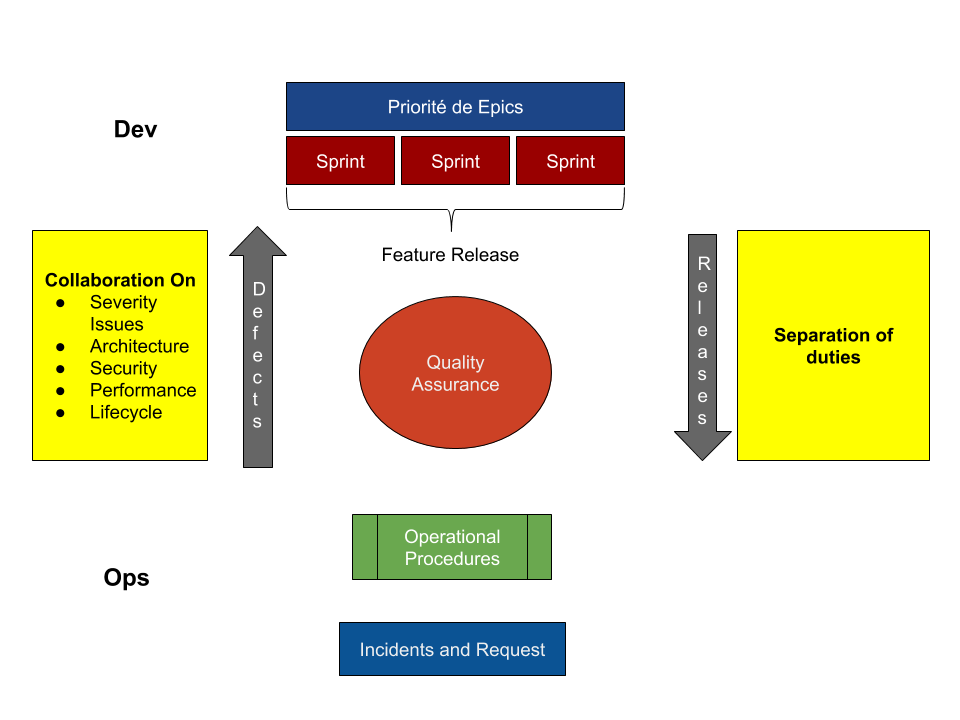
\includegraphics[scale=0.45]{devops_operational_model.png}
\caption{Modèle Opérationnel \cite{IsaacSacolick2016DrivingCulture}}
\label{devops_operational_model}
\end{figure}


\subsubsection{Acteurs}
Dans la Figure \ref{devops_operational_model} nous voyons trois acteur principaux dans cette conversation:

\subparagraph{QA}
C'est une équipe composée par des personnes avec distinctes disciplines qui doivent travailler avec \textit{Dev} pour développer et automatiser les test.
\subparagraph{Dev} L'équipe doit livrer les livrables avec des "runbooks" et d'assurer que les amélioration opérationnelles sont priorité.
\begin{itemize}
  \item Le 30\% d'un sprint doit cibler des défets téchniques.
  \item Cibler le "développement complet", c'est-à-dire, le développement prêt pour les tests de \textit{QA}.
  \item Collabore activement avec \textit{Ops}.
  \item Assurer que l'application récolte des données qui aident à l'amélioration.
\end{itemize}
\subparagraph{Ops}
L'équipe doit fournir des services dans le cloud pour permettre \textit{Dev} être plus agile et lui permettre d'apprendre à résoudre la plupart des problèmes de production.
